
%%%%%%%%%%%%%%%% NÃO ALTERE O CAMPO ABAIXO 
\documentclass[10pt,twoside,a4paper]{article}
\usepackage[T1]{fontenc}
\usepackage[utf8]{inputenc}
\usepackage[portuges]{babel}
\usepackage[a4paper]{geometry}
\geometry{tmargin=1.2cm,bmargin=1.7cm,lmargin=1.5cm,rmargin=1.5cm}
\usepackage{graphicx}
\usepackage{indentfirst}
\usepackage{subcaption} % figuras lado a lado
\usepackage{booktabs} %tabelas
\usepackage{url}% web links
\usepackage{semat}
\usepackage{lipsum} %Texto automático
\usepackage{amsthm, amsmath, amssymb, wasysym, MnSymbol}


\newtheorem{theorem}{Teorema}
\newtheorem{proposition}[theorem]{Proposição}
\newtheorem{lemma}[theorem]{Lema}
\newtheorem{definition}[theorem]{Definição}
\newtheorem{corollary}[theorem]{Corolário}
\renewcommand{\qedsymbol}{$\blacksquare$}


%%%%%%%%%%%%%%%%


%%%%%%%%%%%%%%%% Se necessitar de pacotes adicionais insira abaixo

%\usepackage[•]{•}
%%%%%%%%%%%%%%%%%%%%%%%%%%%%%%%%


%%%%%%%%%%%%%%%%%%
% Não redefina ou crie comandos, por exemplo:
% \R=\mathbb{R} ,\newtheorem{teo}{Teorema}, etc
% Isto pode gerar conflito quando os trabalhos forem
% compilados para o caderno de resumos
%%%%%%%%%%%%%%

%%%%%%%%%%% Não altere os comandos abaixo
\newcommand*{\affaddr}[1]{#1} 
\newcommand*{\affmark}[1][*]{\textsuperscript{#1}}
\newcommand*{\email}[1]{\texttt{#1}}
\usepackage{helvet}% Fonte 
\renewcommand{\familydefault}{\sfdefault}% Fonte 
\renewcommand\Authands{ e }
\evento{XVII Semat e VII Semest}
\date{07 a 10 de novembro de 2017}
%%%%%%%%%%%%%%%%


% Dados do trabalho
\title{Análise numérica de uma discretização explícita da equação da difusão transiente unidimensional.}
% Autores: o primeiro será, necessariamente, o apresentador do trabalho
\author[1]{\underline{Felipe José Oliveira Ribeiro }\thanks{feliperibeiro.ufu@gmail.com}}
\author[1]{Ítalo Augusto Magalhães De Ávila\thanks{italo.ufuracing@gmail.com}}
\author[1]{Hélio Ribeiro Neto\thanks{helio.ribeiro@ufu.br}}
\author[1]{Aristeu da Silveira Neto\thanks{risteus@ufu.br}}
\affil[1]{FEMEC - Universidade Federal de Uberlândia}


%palavras-chave: insira até três palavras
\keywords{Análise numérica. Difusão unidimensional transiente. Diferenças finitas.}

%Compilar o arquivo com PDFLatex
%---------------------------------------------------
\begin{document}
\inserirtitulo
\linespread{1.5}% Espaçamento 1.5
%==================================
% RESUMO
%==================================

\section{Resumo}
No presente trabalho realizar-se-á um estudo de caso do erro numérico na solução da EDP que modela o processo de difusão unidimensional de uma dada informação. 


%==================================
% INTRODUÇÃO
%==================================
\section{Introdução} % apague as linhas abaixo e insira aqui a introdução

A solução numérica de equações diferenciais parciais (EDP’s) é rotineira na modelagem matemática de problemas físicos. Por exemplo, a solução da equação da energia térmica em regime transiente. Em muitos casos, a solução exata é muito complexa, ou mesmo impossível. Para contornar essa barreira, usam-se métodos numéricos (Diferenças finitas, volumes finitos e elementos finitos) que, a partir da discretização espacial e temporal, garantem resultados aproximados. Por não ser um método exato, há formas para quantificar esse erro. No presente trabalho, procura-se apresentar um estudo de caso para a análise de erro envolvendo a resolução da EDP que modela a equação da energia térmica. 

%==================================
% Primeira Seção
%==================================
\section{Método numérico} % apague as linhas abaixo e insira aqui a primeira seção
Na equação da difusão, para o caso unidimensional (indicada abaixo), aparecem duas parcelas diferenciais \cite{Leveque_parabolic}. 
\begin{equation} \label{difusao_pura}
	\frac{\partial \Phi}{\partial t} = \alpha \, \frac{\partial^{2} \Phi}{\partial x^{2}} %+ g\left(x,t\right)
\end{equation}
Na qual $\Phi$ é a variável a ser transportada, que dependente do tempo $t$ e da variável espacial $x$, $\alpha$ é uma constante, a qual pode representar o coeficiente de difusão de
uma dada informação.
Utilizando a expansão em série de Taylor ( equação \ref{serie_taylor}), é possível discretizar os termos no tempo e no espaço para a resolução numérica do problema. 
\begin{equation} \label{serie_taylor}
	\Phi \left(t+\Delta t, x\right)= \Phi \left(t, x\right) + \sum\limits_{n=1}^{\infty} \frac{\Delta t^{n}}{n!} \frac{\partial^{n} \Phi \left(t, x\right)}{\partial t^{n}}
\end{equation}
Para a discretização do termo diferencial de primeira ordem, faz-se uso da relação acima para a expansão da função no domínio do tempo. Logo, para a discretização do termo de primeira ordem no tempo obtém-se a seguinte relação:
\begin{equation} \label{Time_discretization}
\frac{\Phi \left(t+\Delta t, x\right)-\Phi \left(t, x\right)}{\Delta t}= \frac{\partial \Phi \left( x,t \right)}{\partial t} + \sum\limits_{n=2}^{\infty} \frac{\Delta t^{n-1}}{n!} \frac{\partial^{n} \Phi\left(t, x\right)}{\partial t^{n}}
\end{equation}
Truncando-se a equação \ref{Time_discretization} no termo de primeira ordem ($\mathcal{O}(\Delta t)$), obtém-se o método de Euler explícito.
Analogamente, a discretização para o termo de segunda ordem é obtido, fazendo uso de um incremento e um decremento no espaço, enquanto o tempo é fixado.
\begin{equation} \label{Spacial_discretization1}
	\Phi \left(t, x+\Delta x\right)= \Phi \left(t, x\right) \\
	+\sum\limits_{n=1}^{\infty} \frac{\Delta x^{\left(2n-1\right)}}{\left(2n-1\right)!} \frac{\partial^{\left(2n-1\right)} \Phi \left(t, x\right)}{\partial x^{\left(2n-1\right)}}\\
	+\sum\limits_{n=1}^{\infty} \frac{\Delta x^{\left(2n\right)}}{\left(2n\right)!} \frac{\partial^{\left(2n\right)} \Phi \left(t, x\right)}{\partial x^{\left(2n\right)}}
\end{equation}
\begin{equation} \label{Spacial_discretization2}
	\Phi \left(t, x-\Delta x\right)= \Phi \left(t, x\right) \\
	 -\sum\limits_{n=1}^{\infty} \frac{\Delta x^{\left(2n-1\right)}}{\left(2n-1\right)!} \frac{\partial^{\left(2n-1\right)} \Phi \left(t, x\right)}{\partial x^{\left(2n-1\right)}}\\
	 +\sum\limits_{n=1}^{\infty} \frac{\Delta x^{\left(2n\right)}}{\left(2n\right)!} \frac{\partial^{\left(2n\right)} \Phi \left(t, x\right)}{\partial x^{\left(2n\right)}}
\end{equation}
Somando as equações \ref{Spacial_discretization1} e \ref{Spacial_discretization2}, obtém-se a discretização para a derivada segunda no espaço.
\begin{equation} \label{Spacial_discretization3}
\frac{\Phi \left(t, x+\Delta x\right)-2 \Phi \left(t, x\right) + \Phi \left(t, x-\Delta x\right)}{\Delta x^2} = \\
\frac{\partial^{2} \Phi \left(t, x\right)}{\partial x^{2}}+ \\
2 \sum\limits_{n=2}^{\infty} \frac{ \Delta x^{\left(2\left(n-1\right)\right)}}{\left(2n\right)!} \frac{\partial^{\left(2n\right)} \Phi \left(t, x\right)}{\partial x^{\left(2n\right)}}
\end{equation}
Truncando-se a equação \ref{Spacial_discretization3} no termo de segunda ordem ($\mathcal{O}(\Delta x^2)$), obtém-se o método de diferenças centradas.
Substituindo-se as relações truncadas na equação \ref{difusao_pura} tem-se a equação \ref{difusao_discretizada} .
\begin{equation} \label{difusao_discretizada}
\frac{\Phi \left(t+\Delta t, x\right)-\Phi \left(t, x\right)}{\Delta t}\approx \alpha \frac{\Phi \left(t, x+\Delta x\right)-2 \Phi \left(t, x\right) + \Phi \left(t, x-\Delta x\right)}{\Delta x^2}% + g\left(x,t\right)
\end{equation}
Para o desenvolvimento numérico, a discretização temporal e espacial é necessária. Para isso, um domínio contínuo e infinito deve ser traduzido para um conjunto finito e discreto onde se aplica a metodologia numérica. Assim, o domínio é discretizado uniformemente:\\
\\
\begin{minipage}[!h]{0.40\textwidth} 
	\begin{equation}
		t^N = N \Delta t
	\end{equation}
\end{minipage}
\begin{minipage}[!h]{0.40\textwidth}
	\begin{equation}
		x_I = I \Delta x
	\end{equation}
\end{minipage}\\
\\
As variáveis $N$ e $I$ são números inteiros. Dessa forma, defini-se a função numérica com os termos truncados \ref{difusao_discretizada}, como a seguir, no domínio discreto:
\begin{equation}\label{ola}
\frac{\phi ^{N + 1} _ I - \phi ^{N} _ I}{\Delta t} 
=
\alpha \frac{\phi ^{N} _ {I + 1} - 2 \phi ^{N} _ I + \phi ^{N} _ {I-1}}{\Delta x ^ 2} 
\end{equation}
Para se estudar o erro, porém, cria-se uma equação modificada $\Psi (t , x) $. Ela denotaria a relação a cima, ou seja, uma função no contínuo que tem todos os resultados numéricos para o domínio de $\phi ^{N} _ {I}$, para isso, a relação exposta ne equação \ref{ola} precisa ser uma verdade. Assim, expande-se a função $ \Psi (t , x)$ em nos pontos citados na relação em \ref{ola} e desenvolve-se a equação:

\begin{equation} \label{difusao_discretizada_modificada}
\begin{split}
\frac{\Psi (t , x) + \sum\limits_{n=1}^{\infty} \frac{\Delta t^{n}}{n!} \frac{\partial^{n} \Psi (t , x)}{\partial t^{n}} - \Psi (t , x)}{\Delta t} 
=
\alpha \frac{
	\Psi \left(t, x\right)
	+\sum\limits_{n=1}^{\infty} \frac{\Delta x^{\left(2n-1\right)}}{\left(2n-1\right)!} \frac{\partial^{\left(2n-1\right)} \Psi \left(t, x\right)}{\partial x^{\left(2n-1\right)}}
	+\sum\limits_{n=1}^{\infty} \frac{\Delta x^{\left(2n\right)}}{\left(2n\right)!} \frac{\partial^{\left(2n\right)} \Psi \left(t, x\right)}{\partial x^{\left(2n\right)}}
			}{\Delta x ^ 2} \\
-2 \frac{
	\Psi (t , x)
		}{\Delta x ^ 2} + 
\frac{
	\Psi \left(t, x\right) 
	-\sum\limits_{n=1}^{\infty} \frac{\Delta x^{\left(2n-1\right)}}{\left(2n-1\right)!} \frac{\partial^{\left(2n-1\right)} \Psi \left(t, x\right)}{\partial x^{\left(2n-1\right)}}
	+\sum\limits_{n=1}^{\infty} \frac{\Delta x^{\left(2n\right)}}{\left(2n\right)!} \frac{\partial^{\left(2n\right)} \Psi \left(t, x\right)}{\partial x^{\left(2n\right)}}
		}{\Delta x ^ 2}
\end{split}
\end{equation}
\begin{equation}
\begin{split}
\frac{ \sum\limits_{n=1}^{\infty} \frac{\Delta t^{n}}{n!} \frac{\partial^{n} \Psi (t , x)}{\partial t^{n}}}{\Delta t} 
=
2 \alpha \frac{
	\sum\limits_{n=1}^{\infty} \frac{\Delta x^{\left(2n\right)}}{\left(2n\right)!} \frac{\partial^{\left(2n\right)} \Psi \left(t, x\right)}{\partial x^{\left(2n\right)}}
}{\Delta x ^ 2}
\end{split}
\end{equation}
Assim, expandindo-se no primeiro termo obtem-se a equação modificada:
\begin{equation}
\begin{split}
 \frac{\partial \Psi \left(t, x\right) }{\partial t}   + \sum\limits_{n=2}^{\infty} \frac{\Delta t^{n - 1}}{n!} \frac{\partial^{n} \Psi (t , x)}{\partial t^{n}}
= 
\alpha \frac{\partial^2 \Psi \left(t, x\right) }{\partial x^2} +
2 \alpha \sum\limits_{n=2}^{\infty} \frac{\Delta x^{\left(2n - 2\right)}}{\left(2n\right)!} \frac{\partial^{\left(2n\right)} \Psi \left(t, x\right)}{\partial x^{\left(2n\right)}}	
\end{split}
\end{equation}
\begin{equation}\label{olalaaa}
\begin{split}
\frac{\partial \Psi \left(t, x\right) }{\partial t} -
\alpha \frac{\partial^2 \Psi \left(t, x\right) }{\partial x^2} 
= 
2 \alpha \sum\limits_{n=2}^{\infty} \frac{\Delta x^{\left(2n - 2\right)}}{\left(2n\right)!} \frac{\partial^{\left(2n\right)} \Psi \left(t, x\right)}{\partial x^{\left(2n\right)}}
- \sum\limits_{n=2}^{\infty} \frac{\Delta t^{n - 1}}{n!} \frac{\partial^{n} \Psi (t , x)}{\partial t^{n}}	
\end{split}
\end{equation}
Pode-se escrever o passo de tempo em função do passo espacial a partir da definição do CFL (Courant Friedrichs Lewy), da seguinte forma:
\begin{equation} \label{CFL}
\Delta t^n= CFL^n \frac{\Delta x^{2n}}{\alpha^{n}}
\end{equation}
Assim, substituindo esta relação na equação \ref{olalaaa} e truncando-se os termos de ordem superior à quarta:

\begin{equation}
\begin{split}
\frac{\partial \Psi \left(t, x\right) }{\partial t} -
\alpha \frac{\partial^2 \Psi \left(t, x\right) }{\partial x^2} 
= 
2 \alpha \sum\limits_{n=2}^{\infty} \frac{\Delta x^{\left(2n - 2\right)}}{\left(2n\right)!} \frac{\partial^{\left(2n\right)} \Psi \left(t, x\right)}{\partial x^{\left(2n\right)}}
- \sum\limits_{n=2}^{\infty} \frac{\Delta t^{n - 1}}{n!} \frac{\partial^{n} \Psi (t , x)}{\partial t^{n}}	
\end{split}
\end{equation}
\\
. \\ 
. \\
. \\
Utilizando-se o teorema de Clairaut-Schwarz, as derivadas temporais podem ser escritas em função das derivadas espaciais, conforme equação \ref{temp_func_epac}.
\begin{equation} \label{temp_func_epac}
\frac{\partial^{n} \Phi \left( x,t \right)}{\partial t^{n}} =  \alpha^{n} \frac{\partial^{\left(2n\right)} \Phi \left( x,t \right)}{\partial x^{\left(2n\right)}}
\end{equation}
Portanto, substituindo-se a equação \ref{temp_func_epac} na equação \ref{olalaaa}, obtém-se a equação \ref{equacao_modificada}.
\begin{equation} \label{equacao_modificada}
\frac{\partial \Psi \left( x,t \right)}{\partial t} - \alpha \frac{\partial^{2} \Psi \left(t, x\right)}{\partial x^{2}}= 
 \sum\limits_{n=2}^{\infty}\left( \left(\frac{ 2 \alpha \Delta x^{\left(2\left(n-1\right)\right)}}{\left(2n\right)!} -\frac{\Delta t^{n-1} \alpha^{n}}{n!}\right) \frac{\partial^{\left(2n\right)} \Phi \left(t, x\right)}{\partial x^{\left(2n\right)}}\right)
\end{equation}
Pode-se escrever o passo de tempo em função do passo espacial da seguinte forma:
\begin{equation} 
\Delta t^n= CFL^n \frac{\Delta x^{2n}}{\alpha^{n}}
\end{equation}
Na qual $CFL$ é uma constante. Substituindo-se a equação \ref{CFL} na equação \ref{equacao_modificada}, tem-se:
\begin{equation} \label{equacao_modificadaCFL}
\frac{\partial \Phi \left( x,t \right)}{\partial t} = \alpha \frac{\partial^{2} \Phi \left(t, x\right)}{\partial x^{2}}+ \\
\sum\limits_{n=2}^{\infty}\left( \left(\frac{ 2  }{\left(2n\right)!} -\frac{CFL^{\left(n-1\right)}  }{n!}\right) \alpha \Delta x^{\left(2\left(n-1\right)\right)} \frac{\partial^{\left(2n\right)} \Phi \left(t, x\right)}{\partial x^{\left(2n\right)}}\right)
\end{equation}
Para cada $n$ existe um valor de $CFL$ que zera o erro de ordem  $\mathcal{O}\left(\Delta x^{\left(2\left(n-1\right)\right)}\right)$ conforme equação \ref{CFLn}.
\begin{equation} \label{CFLn}
CFL_o\left(n\right)=\left(\frac{2 \, n!}{(2n)!}\right)^\frac{1}{n-1}.
\end{equation}
Na qual $CFL_o\left(n\right)$ é o valor de $CFL$ que zera o erro de ordem  $\mathcal{O}\left(\Delta x^{\left(2\left(n-1\right)\right)}\right)$. Pode-se avaliar o valor de $CFL_o\left(n\right)$ para n=2:
\begin{equation} \label{CFL_otimo}
CFL_o\left(2\right)=\left(\frac{1}{6}\right)
\end{equation}
Portanto, o erro de ordem $\mathcal{O}(\Delta x^2)$ some se $CFL=$ 1/6. Dessa forma, o erro $\mathcal{O}(\Delta x^4)$ passa a ser o erro de mais baixa ordem do método. Para outros valores de $CFL$ o erro do método é de segunda ordem.
%==================================
% Segunda Seção
%==================================
\section{Estudo de caso} % apague as linhas abaixo e insira aqui a segunda seção

Para a solução da equação \ref{difusao_discretizada} são necessárias condições de contorno, condição inicial, domínio espacial e tempo final de simulação. Para esse estudo de caso, a condição inicial imposta foi:
\begin{equation} \label{condicao_inicial}
\Phi(0,x)=U_0 \sin\left(\theta x\right), %e^{-\alpha \theta^2 t},
\end{equation}
na qual $U_0$ é a amplitude da função e $\theta$ é o número de onda. As condições de contorno foram:
\begin{equation} \label{condicoes_contorno}
\begin{split}
\Phi(0,0)&=0,\\
\Phi(0,2\pi)&=0.
\end{split}
\end{equation}
O domínio espacial escolhido foi de $x=[0,2\pi]$ o tempo final de simulação foi de $50$ segundos.
Para determinar o erro e a convergência do método, comparou-se a solução numérica com a solução analítica:
\begin{equation} \label{solucao_analitica}
\Phi(t,x)=U_0 \sin\left(\theta x\right) e^{-\alpha \theta^2 t},
\end{equation}
As variáveis $U_0$, $\theta$ e $\alpha$ foram impostas como $1$. A determinação do erro numérico foi feita para $CFL=$ 0,5 (Tabela \ref{tabela1}) e para $CFL=$ 1/6 (Tabela \ref{tabela2}). Variou-se o número de nós espaciais para verificar a influência do $\Delta x$ no erro numérico. Na coluna "Razão", para 100 nós espaciais, foi determinada a razão entre o erro com 50 nós espaciais e o erro com 100 nós e assim por diante. Para o cálculo da ordem, foi feito o cálculo do logaritmo da razão na base 2, visto que o número de nós espaciais dobra em relação à simulação anterior. Como esperado, foram observadas ordem 2 e 4 para $CFL=$ 0,5 e $CFL=$ 1/6, respectivamente.

\begin{table}[h!]
\caption{Erro do método numérico para $CFL$=0,5.}
\label{tabela1}
\centering
\begin{tabular}{cccc}
\hline
Número de nós  espaciais&        Erro $L_\infty$       & Razão      & Ordem    \\ \hline
$50$ &       $2,31 \, 10^{-5}$        & $---$      & $---$    \\ 
$100$ &       $5,66 \, 10^{-6}$        & $4,08$      & $2,03$    \\ 
$200$ &       $1,40 \, 10^{-6}$        & $4,04$      & $2,01$    \\ 
$400$ &       $3,48 \, 10^{-7}$        & $4.02$      & $2.01$    \\ \hline
\end{tabular}
\end{table}

\begin{table}[h!]
\caption{Erro do método numérico para $CFL$=1/6.}
\label{tabela2}
\centering
\begin{tabular}{cccc}
	\hline
	Número de nós espaciais &        Erro $L_\infty$       & Razão      & Ordem    \\ \hline
	$50$ &       $1,05 \, 10^{-9}$        & $---$      & $---$    \\ 
	$100$ &       $6,33 \, 10^{-11}$        & $16,59$      & $4,05$    \\ 
	$200$ &       $3,85 \, 10^{-12}$   & $16,44$      & $4,04$    \\ 
	$400$ &       $2,40 \, 10^{-13}$        & $16,04$      & $4,00$    \\ \hline
\end{tabular}
\end{table}

Além da análise da convergência do método, foi feita a análise do erro variando-se o $CFL$. O passo de tempo foi mantido constante em $10^{-4}$ s e em cada simulação foram feitos 100 passos temporais. O número de nós espaciais utilizados variou de 20 até 525. A figura \ref{fig:erro} mostra o erro numérico das simulações variando-se o $CFL$. Como esperado, o menor erro acontece quando o $CFL=$ 1/6. É importante notar que para $CFL$ maior ou igual a 0,5 o método se torna instável \cite{Leveque_parabolic}. No caso simulado, o $CFL$ no qual o método se mostrou instável foi de 0,5572. Isso aconteceu porque foram simulados somente 100 passos no tempo, que não foram suficientes para que o método se mostrasse instável. Se mais passos temporais forem realizados, o método se mostrará instável para $CFL=$ 0,5.

\begin{figure}[!hbt]
\centering
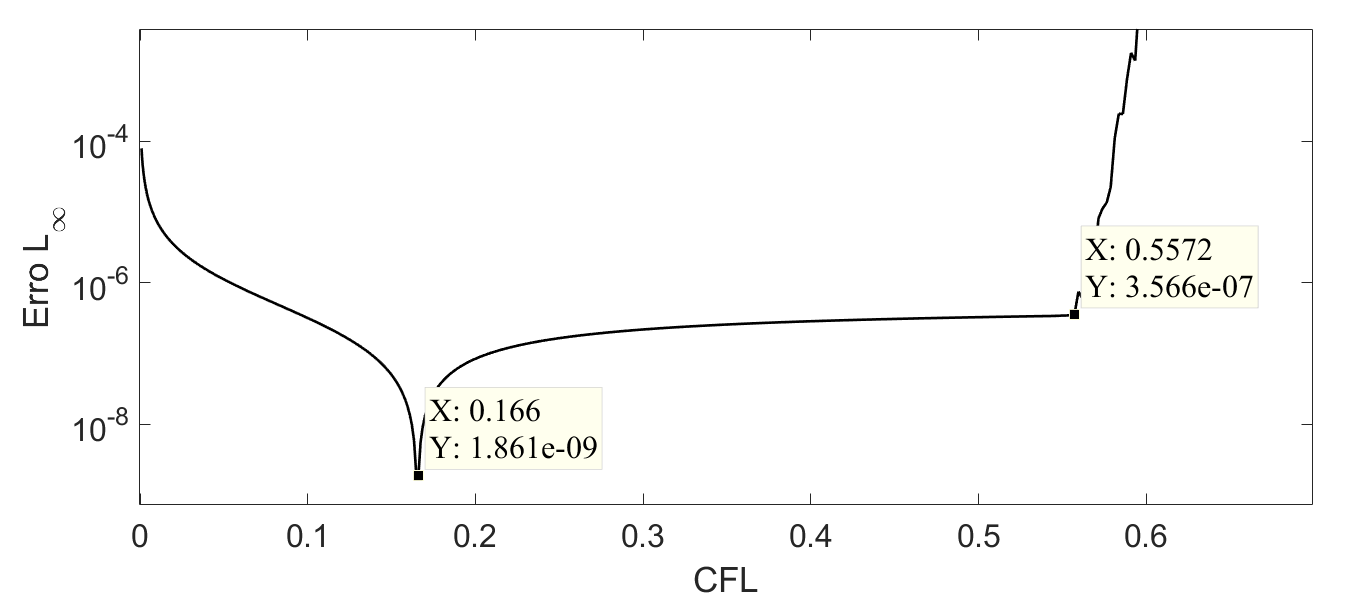
\includegraphics[scale=0.4]{semat_fig2}
\caption{Erro numérico das simulações em função do $CFL$.}
\label{fig:erro}
\end{figure}

%==================================
% CONCLUSÃO
%==================================
\section{Conclusão} % apague as linhas abaixo e insira aqui a conclusão
Propôs-se a avaliação do erro numérico para a solução numérica da equação diferencial parcial parabólica que modela o
processo transiente de difusão unidimensional de uma dada informação. Para isso, fez-se uso do método de diferenças finitas para discretizar as equações. Utilizou-se o método de Euler explícito para a derivada parcial temporal e diferenças centradas para a espacial. Foram feitas a análise numérica do método de discretização e simulações computacionais para avaliar o erro numérico. A solução computacional foi comparada com a solução analítica.

Conclui-se que existe uma relação entre o passo de tempo, o passo espacial e o coeficiente de difusão que minimiza o erro numérico. Essa relação foi chamada de $CFL$ e o valor ótimo desse parâmetro para a diminuição do erro é de 1/6. Mostrou-se também, que a ordem do erro de discretização com esse $CFL$ ótimo foi de $\mathcal{O}(\Delta x^4)$, enquanto para outros valores de $CFL$ a ordem do método é de $\mathcal{O}(\Delta x^2)$.


%==================================
% AGRADECIMENTOS
%==================================
\section{Agradecimentos} % apague as linhas abaixo e insira aqui os agradecimentos

Os autores gostariam de agradecer à Petrobras, CAPES, FAPEMIG, CNPq, MFLab e à FEMEC/UFU pelo suporte no desenvolvimento do presente trabalho. 

%==================================
% REFERÊNCIAS
%==================================

\begin{thebibliography}{9} % apague as linhas abaixo e insira aqui bibliografia

\bibitem{Leveque_parabolic}
	LeVeque, R. J.,
	2007,
	\emph{Finite difference methods for ordinary and partial differential equations : steady-state and
		time-dependent problem},
	1ª edição,
	University City Science Center, Philadelphia, United States:
	SIAM, 2007. 357 páginas. (Classics in Applied Mathematics)
\end{thebibliography}

%--- FIM ---
\end{document}
